\chapter{Concept of our solution} %\label{cha:eva}}
In this chapter we will introduce the initial proposed solution. Some preliminary experiments will be presented, as well as plan for the future work.
\section{Proposed solution}

\begin{figure}[!ht]
\begin{centering}
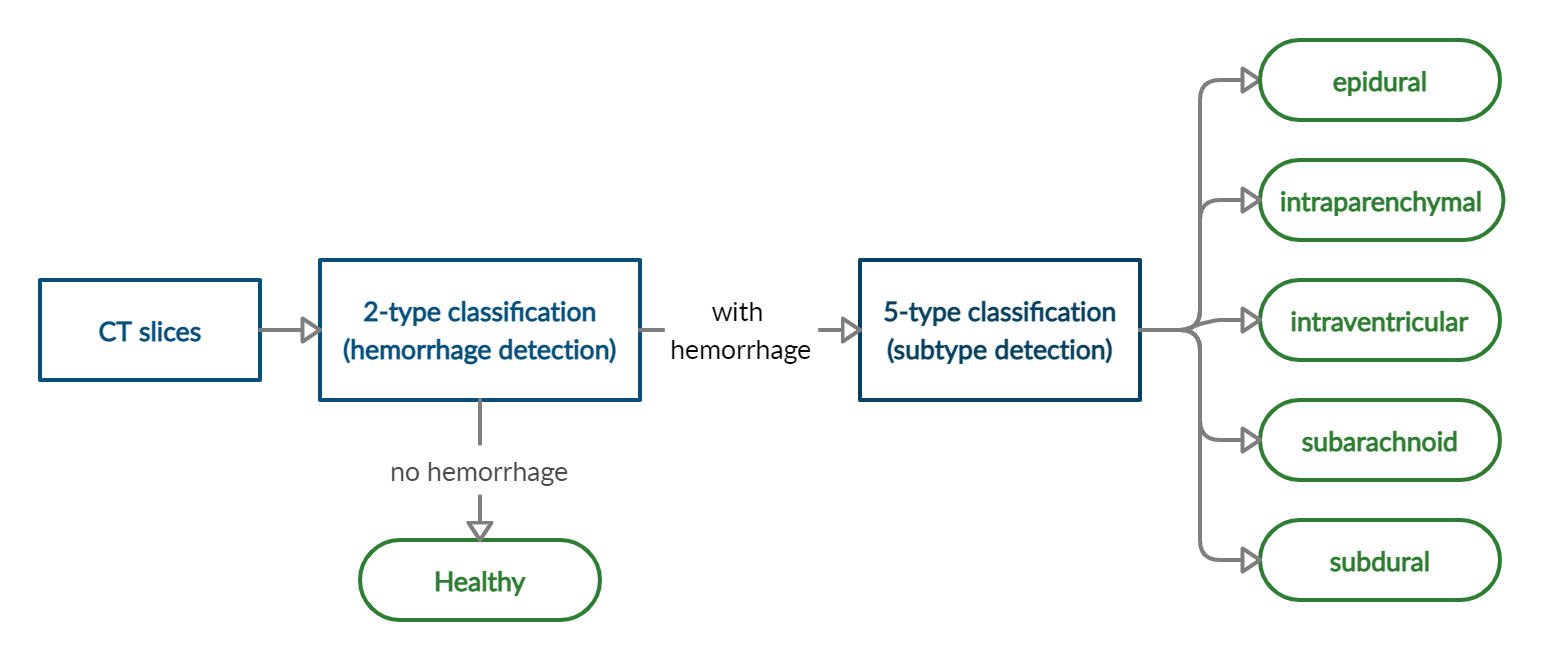
\includegraphics[width=16cm]{assets/images/mySolution.png}
\par\end{centering}
\caption{Diagram of proposed solution \label{fig:solution}}
\end{figure}

\section{Our dataset}
In our work, we use a dataset provided by the Radiological Society of North America (RSNA)  \cite{RSNAchallenge}. The data was collected from four research institutions (Stanford University, Thomas Jefferson University, Unity Health Toronto and Universidade Federal de São Paulo) and put together for the RSNA Intracranial Hemorrhage Detection Challenge 2019, which was a competition held on the Kaggle platform\footnote{https://www.kaggle.com/c/rsna-intracranial-hemorrhage-detection/overview}. The dataset consists of training and testing set, which contain 752,803 and 121,232 individual CT slices respectively. A team of 60 radiology volunteers labeled the CT examinations according to the five intracranial hemorrhage subtypes - epidural (EPH), intraparenchymal (IPH), intraventricular (IVH), subarachnoid (SAH), subdural (SDH). Additional label named "any" is provided to indicate if any type of hemorrhage is present in the CT slice. Annotations are at disposal in a table format inside the corresponding csv file. All provided CT slices are in the DICOM (Digital Imaging and Communications in Medicine) format, which is the standard format for storing and transferring medical data. Along with the image contains this format also associated metadata, such as PatientID, StudyInstanceUID, SeriesInstanceUID and other. Even though the data is provided as individual CT scans, these can be grouped to form original CT scan by the ScanID, which can be found in the DICOM metadata. Each slice is a 16-bit grayscale image and has the spatial dimensions of 512x512 pixels. 
\begin{figure}[!ht]
\begin{centering}
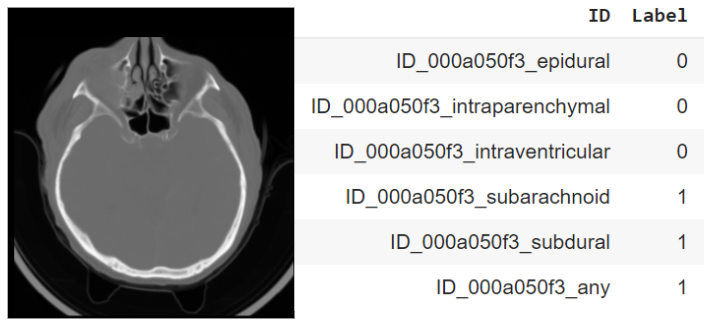
\includegraphics[width=10cm]{assets/images/datasetExample}
\par\end{centering}
\caption{Example CT slice and corresponding annotation from the dataset \label{fig:dataset}}
\end{figure}

\section{Future work}
